\documentclass[12pt, openany]{article}
\usepackage[utf8]{inputenc}
\usepackage[T1]{fontenc}
\usepackage[a4paper,left=2cm,right=2cm,top=2cm,bottom=2cm]{geometry}
\usepackage[frenchb]{babel}
\usepackage{libertine}
\usepackage[pdftex]{graphicx}

\setlength{\parindent}{0cm}
\setlength{\parskip}{1ex plus 0.5ex minus 0.2ex}
\newcommand{\hsp}{\hspace{20pt}}
\newcommand{\HRule}{\rule{\linewidth}{0.5mm}}

\begin{document}

\begin{titlepage}
  \begin{sffamily}
  \begin{center}

    % Upper part of the page. The '~' is needed because \\
    % only works if a paragraph has started.
    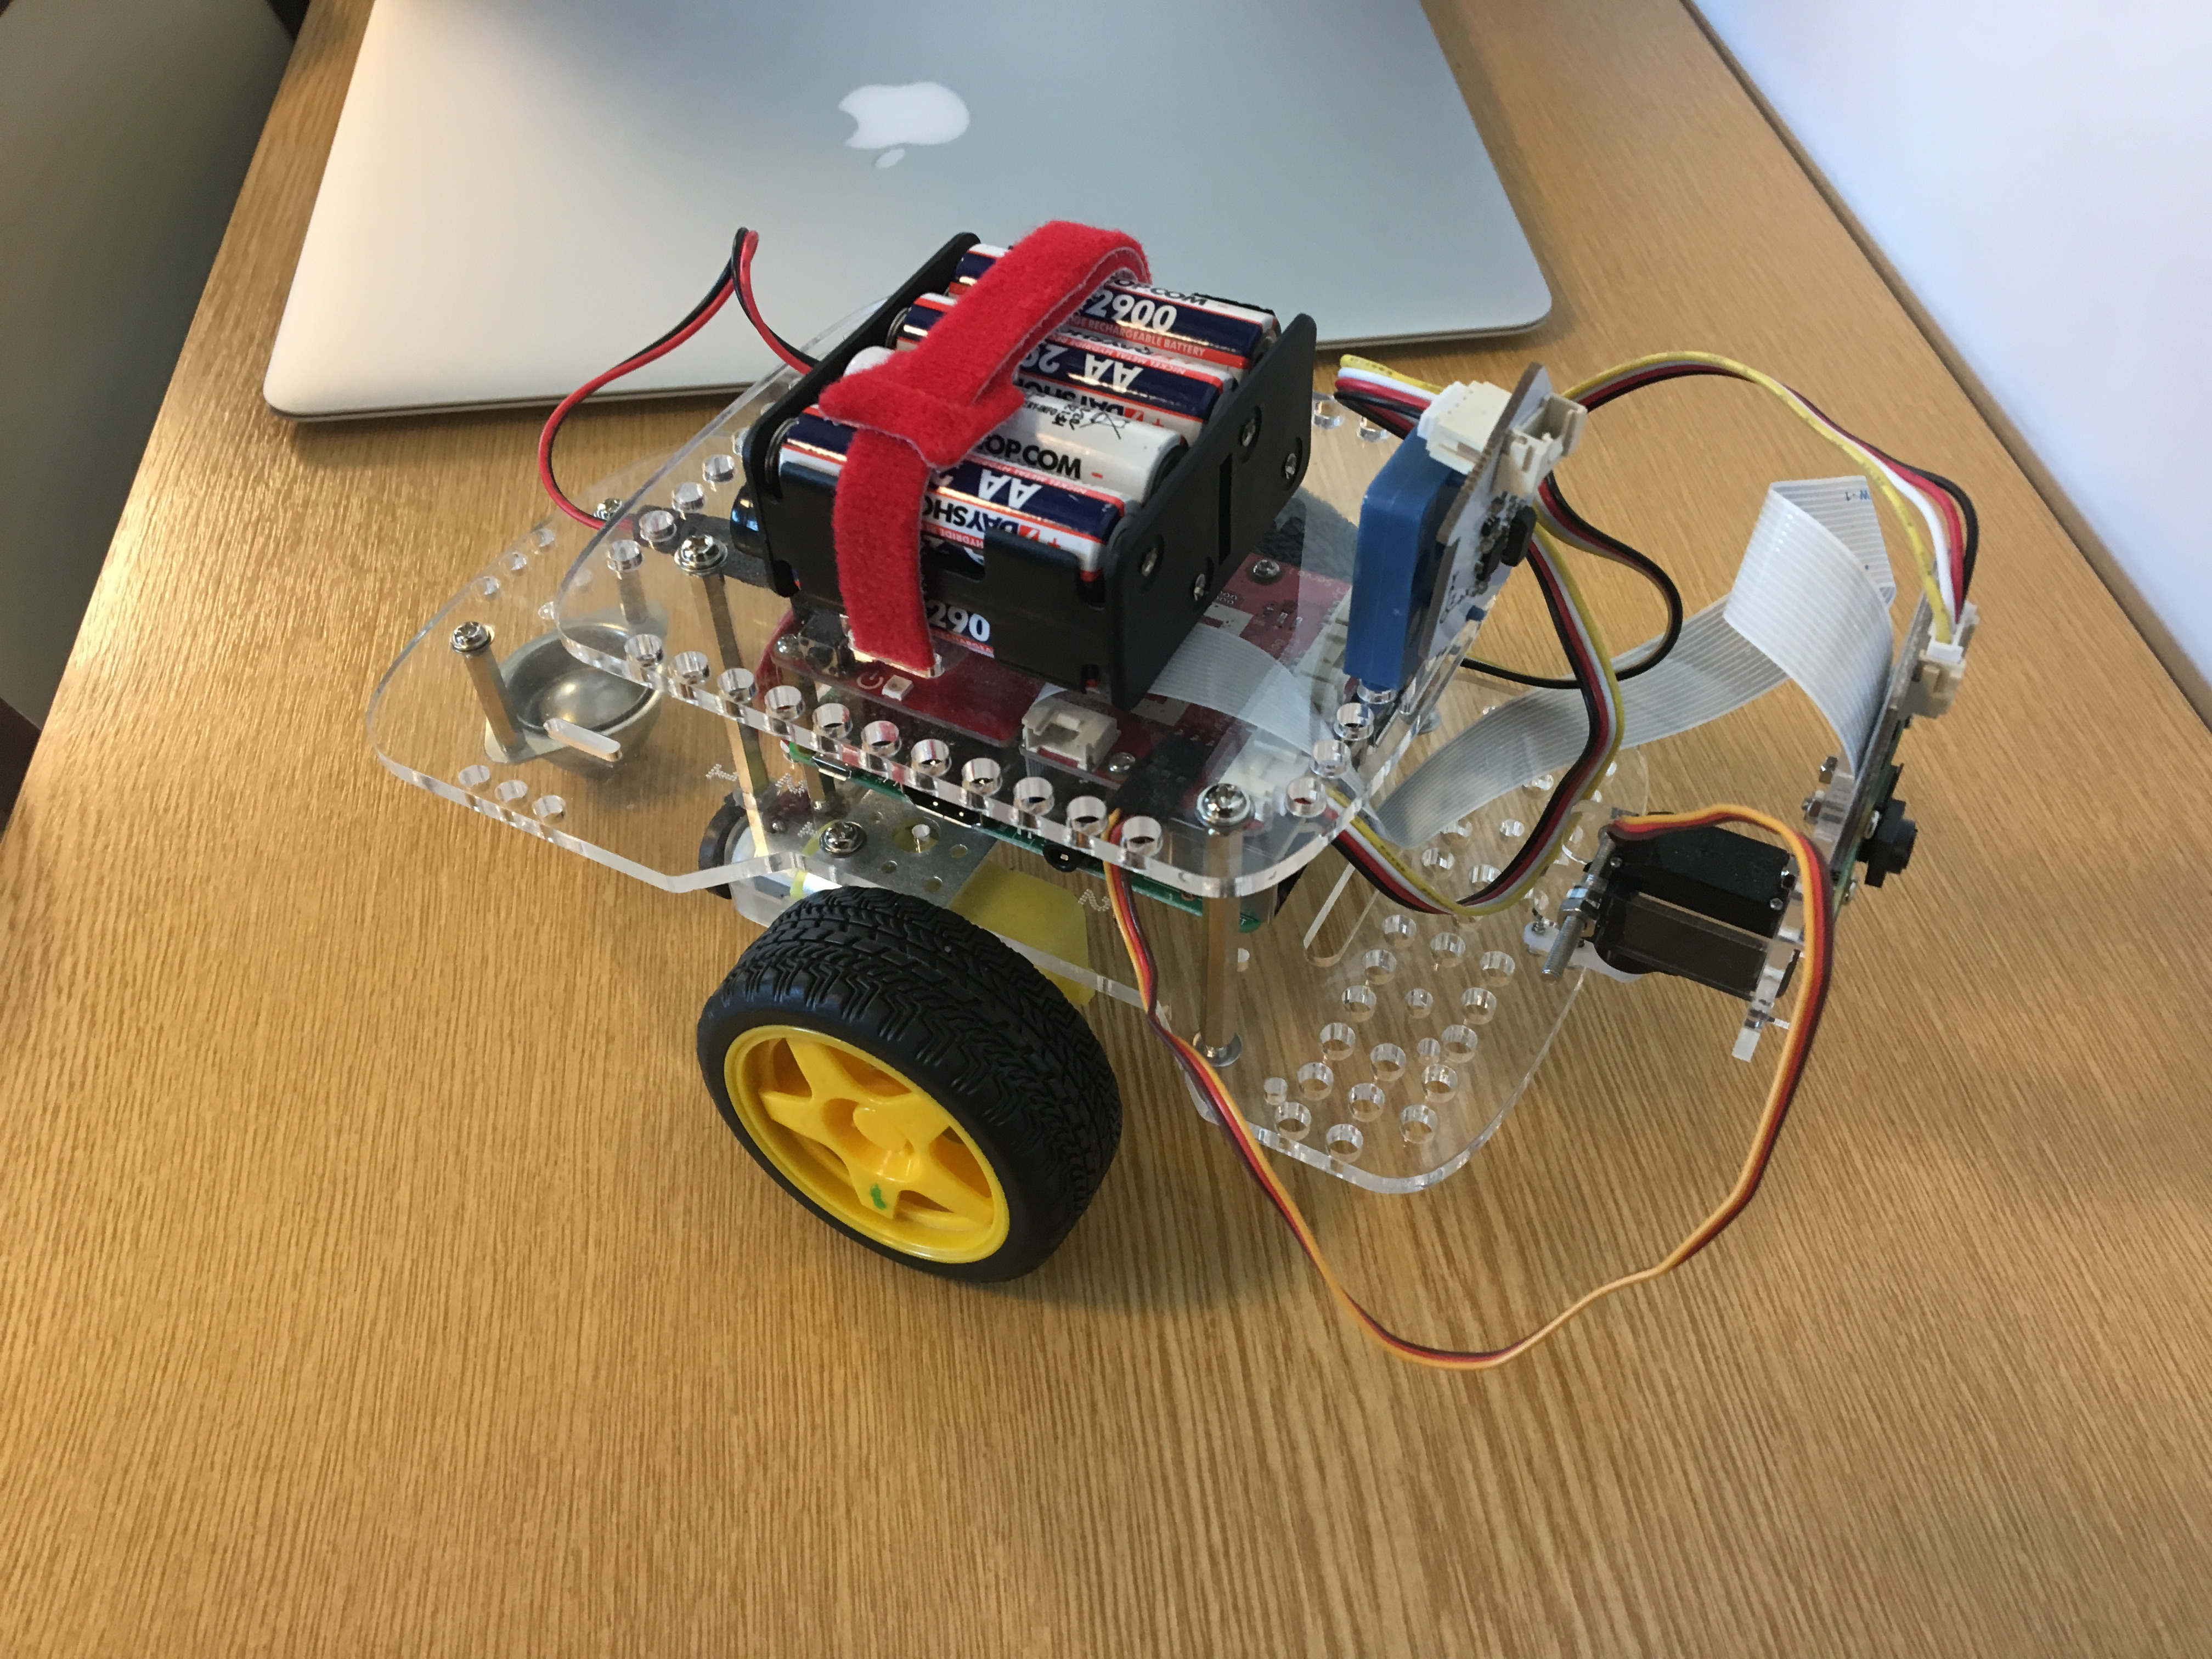
\includegraphics[scale=0.04]{IMG_8579.JPG}~\\[1cm]

    \textsc{\LARGE Sorbonne Université}\\[1cm]

    \textsc{\Large Rapport de projet}\\[1.5cm]

    % Title
    \HRule \\[0.4cm]
    { \huge \bfseries Projet Robotique\\[0.4cm] }

    \HRule \\[1cm]
    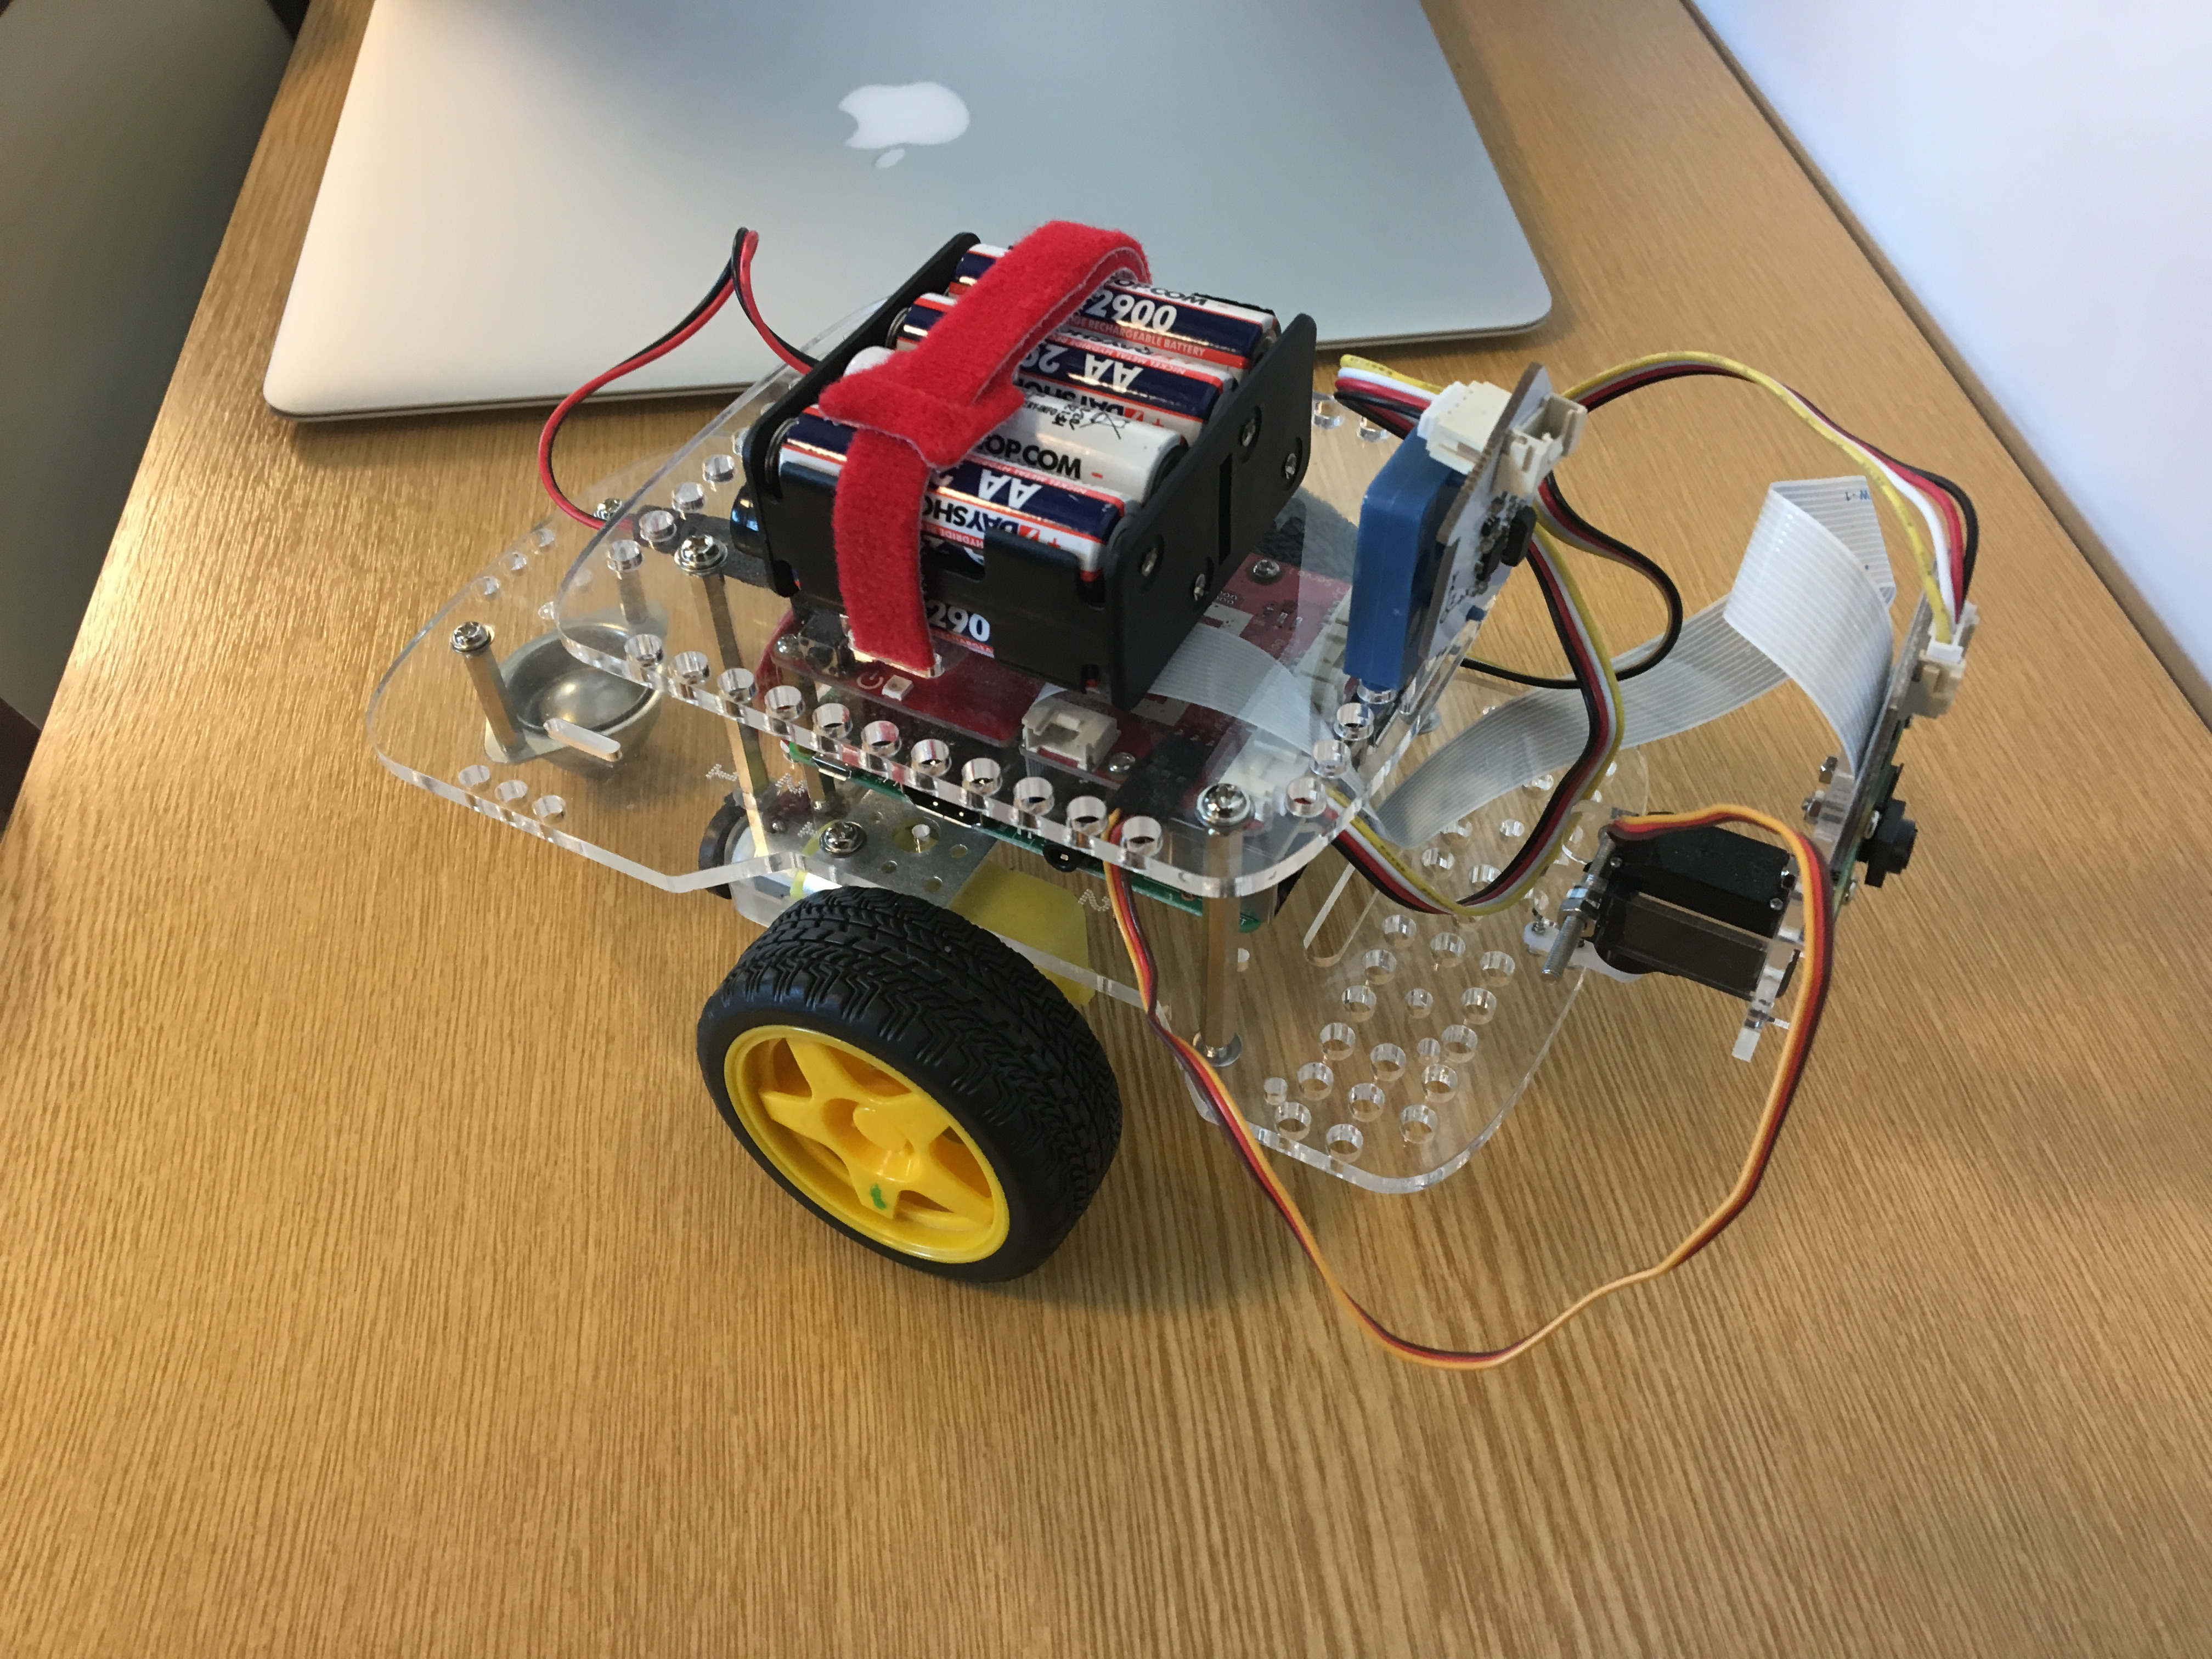
\includegraphics[scale=0.1]{IMG_8579.JPG}
    \\[0.5cm]

    % Author and supervisor
    \begin{minipage}{0.4\textwidth}
      \begin{flushleft} \large
        Groupe \textsc{FiveGuys}\\
        UE 2I013\\
      \end{flushleft}
    \end{minipage}
    \begin{minipage}{0.4\textwidth}
      \begin{flushright} \large
        \emph{Chargé de cours:} M. \textsc{Baskiotis}\\
        \emph{Chargé de TME:} M. \textsc{Veniat}
      \end{flushright}
    \end{minipage}

    \vfill

    % Bottom of the page
    {\large 1\ier{} Février 2019 — Mai 2019}

  \end{center}
  \end{sffamily}
\end{titlepage}

\tableofcontents
\newpage

\section{Introduction}
Dans le cadre de l'UE 2I013, notre projet était de concevoir un logiciel permettant de contrôler un robot. Le projet était entièrement à notre charge aucun code ne nous était fourni.

L'objectif principal de ce projet était d'une part d'être un premier contact avec un projet de robotique et une découverte

Dans un premier temps, l'objectif est de mettre en place les briques de bases de notre projet comme le simulateur 2D et le moddèle physique ainsi que de mettre en place nos outils pour le bon déroulement du travail de groupe.

Dans un second temps, une fois que notre modèle physique et notre simulateur étaient consédéré suffisament stable, nous avons commencé à développer les stratégies qui nous permettent de répondre aux challenges qui nous ont été soumis.
%Dans un premier temps, il a fallu que mettions en place les outils utiles à l'organisation du travail de groupe ainsi qu'une première idée générale de la façon dont nous allions organiser notre projet. Dans un deuxième temps nous avions pour objectif de créer un simulateur et un modèle physique représentatif du réel afin de tester les fonctionnalités que nous souhaitions implémenter dans le robot.
\section{Rapport}
\subsection{Partie 1}
\subsubsection{Sous partie 1}
\subsection{Partie 2}
\subsection{Partie 3}
\section{Remerciements}
\section{Conclusion}
\end{document}
